%%%%%%%%%%%%%%%%%%%%%%%%%%%%%%%%%%%%%%%%%
% Apps tooling for BQNT Apps presentation
% Version 1.0 (01/31/19)
%
% This template has been downloaded from:
% http://www.LaTeXTemplates.com
%
% License:
% CC BY-NC-SA 3.0 (http://creativecommons.org/licenses/by-nc-sa/3.0/)
%
%%%%%%%%%%%%%%%%%%%%%%%%%%%%%%%%%%%%%%%%%

%----------------------------------------------------------------------------------------
%	PACKAGES AND THEMES
%----------------------------------------------------------------------------------------

\documentclass{beamer}

\mode<presentation> {

% The Beamer class comes with a number of default slide themes
% which change the colors and layouts of slides. Below this is a list
% of all the themes, uncomment each in turn to see what they look like.

%\usetheme{default}
%\usetheme{Marburg}
\usetheme{Singapore}

% As well as themes, the Beamer class has a number of color themes
% for any slide theme. Uncomment each of these in turn to see how it
% changes the colors of your current slide theme.

%\usecolortheme{beaver}
%\usecolortheme{crane}
%\usecolortheme{dolphin}
\usecolortheme{dove} 
%\usecolortheme{lily}
%\usecolortheme{wolverine}

%\setbeamertemplate{footline} % To remove the footer line in all slides uncomment this line
%\setbeamertemplate{footline}[page number] % To replace the footer line in all slides with a simple slide count uncomment this line

%\setbeamertemplate{navigation symbols}{} % To remove the navigation symbols from the bottom of all slides uncomment this line
}

\usepackage{graphicx} % Allows including images
\usepackage{booktabs} % Allows the use of \toprule, \midrule and \bottomrule in tables

%----------------------------------------------------------------------------------------
%	TITLE PAGE
%----------------------------------------------------------------------------------------

\title[Short title]{App Framework definition for BQNT} % The short title appears at the bottom of every slide, the full title is only on the title page

\author{Alex} % Your name
\institute[Bloomberg LP] % Your institution as it will appear on the bottom of every slide, may be shorthand to save space
{
\medskip
\textit{Bloomberg LP} % Your email address
}
\date{\today} % Date, can be changed to a custom date

\begin{document}

\begin{frame}
\titlepage % Print the title page as the first slide
\end{frame}

\begin{frame}
\frametitle{Agenda} % Table of contents slide, comment this block out to remove it
\tableofcontents % Throughout your presentation, if you choose to use \section{} and \subsection{} commands, these will automatically be printed on this slide as an overview of your presentation
\end{frame}

%----------------------------------------------------------------------------------------
%	PRESENTATION SLIDES
%----------------------------------------------------------------------------------------

%------------------------------------------------
\section{Project Overview} % Sections can be created in order to organize your presentation into discrete blocks, all sections and subsections are automatically printed in the table of contents as an overview of the talk
%------------------------------------------------

%\subsection{Subsection Example} % A subsection can be created just before a set of slides with a common theme to further break down your presentation into chunks

\begin{frame}
\frametitle{Project Overview}
\begin{itemize}
\item Speed up the development process.
\item Stop duplicating the work on each desk.
\item Access and read someone else's code without training.
\item Pick-up modules/portions of code to reuse in your own App developments.
\end{itemize}
\end{frame}

%------------------------------------------------
\section{Standard Framework}
%------------------------------------------------

\begin{frame}
\frametitle{Standard Framework}

Model development for Apps will be based on MVC Model-View-Controller. \\~\\
Model-View-Controller is an architectural pattern commonly used for developing user interfaces that divides an application into three interconnected parts. This is done to separate internal representations of information from the ways information is presented to and accepted from the user. The MVC design pattern decouples these major components allowing for efficient code reuse and parallel development.

\end{frame}

\begin{frame}
\frametitle{Standard Framework}

\begin{figure}
    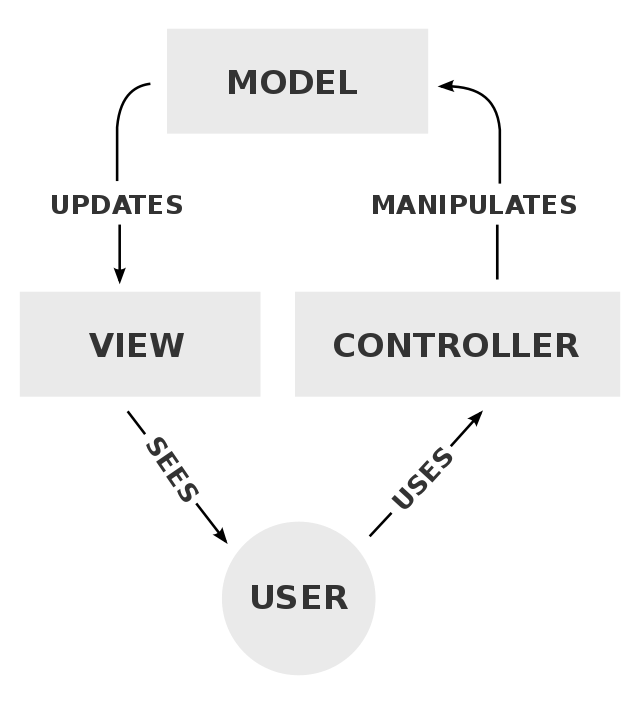
\includegraphics[width=0.7\columnwidth]{images/MVC-Process.png}
    \caption{Diagram of interactions within the MVC pattern.}
\end{figure}

\end{frame}

%------------------------------------------------

\begin{frame}
\frametitle{Adapting to BQNT Apps}
\begin{block}{Model: model.py}
Source code file that invoke the bql library and receives user inputs to customize the data requests from BQL. This file also transforms the dataset in the right shape to match the objects requirements (defined timeseries for Line chart, 2-axis matrix for GridHeatMap chart, etc.).
\end{block}

\begin{block}{View: app.py}
Source code file that invoke the graphical and visual libraries (bqplot, ipywidgets, bqwidgets). Design the UI and call the model functions to populate objects with data.
\end{block}

\begin{block}{Controller: main.ipynb}
Interactive Python notebook that initiates the class of the App.
\end{block}
\end{frame}


\begin{frame}
\frametitle{Adapting to BQNT Apps}

\begin{figure}
    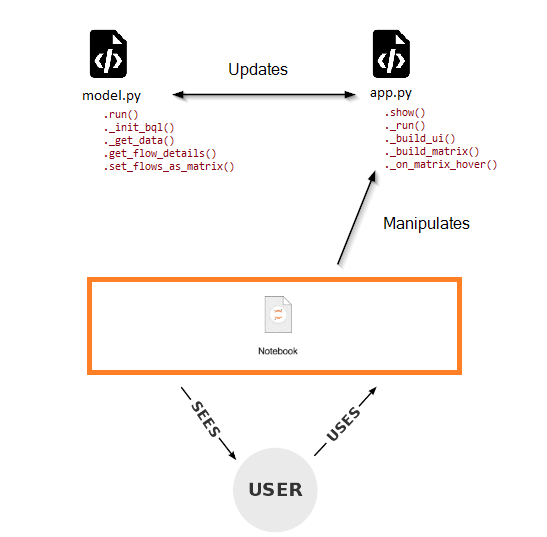
\includegraphics[width=0.7\columnwidth]{images/MVC-Process_BQNT.png}
    \caption{Diagram of interactions within the BQNT App.}
\end{figure}

\end{frame}


\begin{frame}
\frametitle{Adapting to BQNT Apps}

\begin{figure}
    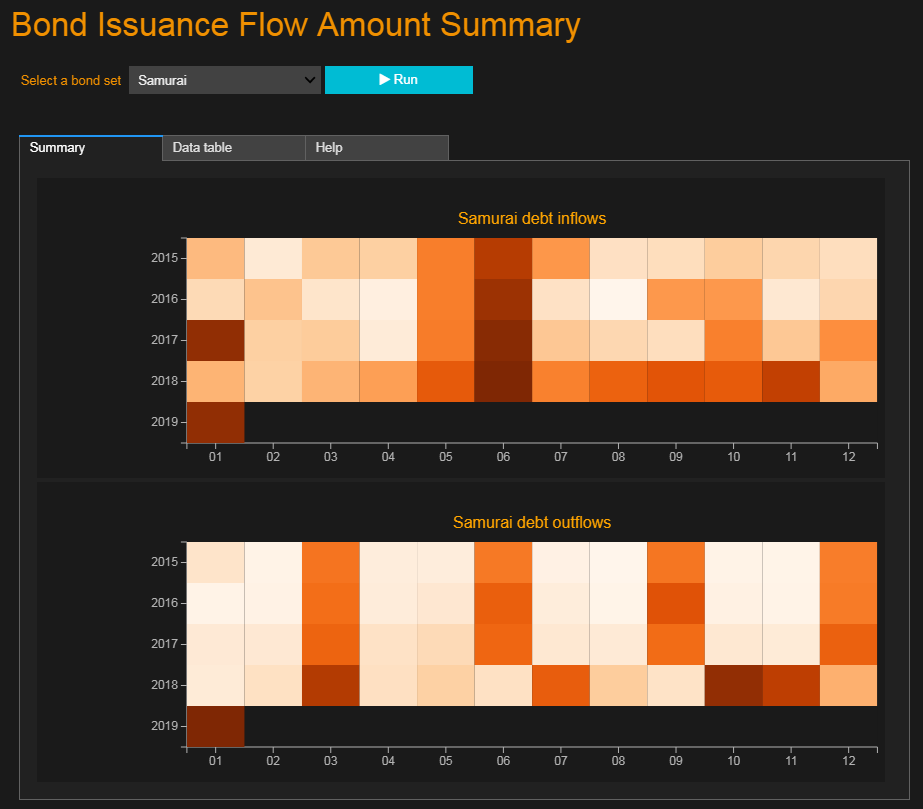
\includegraphics[width=0.7\columnwidth]{images/HeatMapApp.png}
    \caption{Result of the UI BQNT App.}
\end{figure}

\end{frame}

%------------------------------------------------


\begin{frame}
\frametitle{Contributing}
\begin{block}{Github}
https://bbgithub.dev.bloomberg.com/DesktopBuildGroup
\end{block}

\begin{block}{Readme file}
Needs to contain the following for proper documentation
\begin{itemize}
\item App description
\item Top key feature/selling point
\item Target players/users
\item video (optional, but way more efficient)
\end{itemize}
\end{block}

\end{frame}

%------------------------------------------------

\begin{frame}
\Huge{\centerline{End}}
\end{frame}

%----------------------------------------------------------------------------------------

\end{document}